\section{Background and Preliminaries} \label{BRW}

\subsection{Related Work}
\noindent \textbf{Diffusion for Molecular Graphs (Unconditional / Property-based):}
Diffusion models are widely used for molecular graph generation, spanning unconditional sampling and property-conditioned design. Recent variants improve expressivity via transformer-style graph denoisers \citep{liu2024graphdit}, explore hierarchical/latent formulations for scalability and structure preservation \citep{bian2024hglatentdiff}, and study control mechanisms for property prediction and guidance \citep{zhang2025mgdiff}.

\noindent \textbf{Text-guided Molecule Generation:}
Text-to-molecule generation is typically formulated as learning $p(\tilde{\mathcal{G}}\mid \mathbf{S})$ (or $p(\text{SMILES}\mid \mathbf{S})$), where $\mathbf{S}$ describes desired structure or function. Recent work adapts PLMs to chemical strings, enabling text$\leftrightarrow$molecule translation with encoder--decoder pretraining \citep{edwards-etal-2022-translation} and improved multi-task / chemistry-aware extensions \citep{kim2025camt5}. In parallel, diffusion-based text conditioning has emerged, including diffusion-LM style text-guided generation in discrete/embedded sequence spaces \citep{gong2024tgmdlm} and graph/latent diffusion variants that preserve molecular structure \citep{chang2025ldmoltexttomoleculediffusionmodel}.

\noindent \textbf{Molecule Captioning / Molecule-to-Text:}
Generating faithful descriptions from molecules (G2S) has been explored via translation-style baselines \citep{edwards-etal-2022-translation} and molecule captioning models that incorporate structural encoders to improve grounding \citep{liu2024molcamoleculargraphlanguagemodeling}. More recent multimodal approaches further strengthen molecule--language alignment for captioning and related tasks.

\noindent \textbf{Unifying / Bidirectional Molecule--Text Modeling:}
While text-guided generation and captioning have progressed independently, \emph{fully bidirectional} modeling that supports both $p(\mathbf{S}\mid \tilde{\mathcal{G}})$ and $p(\tilde{\mathcal{G}}\mid \mathbf{S})$ within a single generation framework remains relatively limited. Translation-based PLM systems offer practical bidirectionality \citep{edwards-etal-2022-translation}, and recent foundation-model efforts move toward broader cross-modal generalization \citep{liu2024molcamoleculargraphlanguagemodeling}, but diffusion-based approaches are typically developed for one direction (most often S2G) and do not explicitly address token-level corruption heterogeneity. \texttt{BiMol-Diff} fills this gap by casting \emph{both} directions under a unified conditional diffusion view and introducing a molecular graph-aware, token-dependent noising schedule to preserve chemically salient information during generation (see Appendix~\ref{related work}).

%%%%%%%%%%%%%%%%%%%%%%%%%%%
% Recent advances in molecular graph–language modeling cover both graph-to-text (e.g., molecular description) and text-to-graph (e.g., molecule generation) tasks. Graph-to-text has evolved from rule-based methods to neural models with GNNs and pretrained transformers, yielding more fluent, generalizable outputs~\cite{edwards-etal-2022-translation}. Text-to-graph generation remains challenging for preserving molecular structure, semantic alignment, and coherence~\cite{edwards2024molcap, zhang2025atomas}, motivating unified graph-conditioned diffusion approaches.

%%%%%%%%%%%%%%%%%%%%%%%%%%%


% \noindent \textbf{Diffusion Models for Molecular and Language Generation}: Diffusion-based generative models have shown promise in molecular generation and language\cite{liu2023multi}. In molecules, they support both 2D and 3D structure generation with improved diversity and validity compared to autoregressive models \cite{xu2022geodiff}. For text, diffusion language models (DLMs) offer iterative refinement over noisy sequences, countering limitations such as exposure bias and mode collapse in transformer decoders \cite{li2022diffusionlmimprovescontrollabletext, nie2025large}. Despite their individual success, the integration of graph-conditioned diffusion models for joint molecule generation and description remains largely unexplored.

% \noindent \textbf{Bridging Molecular Design and Description}: Current models typically treat molecule generation and description as separate tasks, structure-first generation followed by annotation, or text-conditioned generation without structural grounding. In this paper, we present a unified graph-conditioned diffusion framework that jointly models molecular design and its semantic explanation. This addresses a significant gap in multimodal generative chemistry and provides a flexible tool for structure-aware molecular language tasks.
%%%%%%%%%%%%%%%%%%%%%%%%%%%%%%%%%%%%%%%%%
\subsection{Preliminaries}
\begin{figure*}[t!]
    \centering
    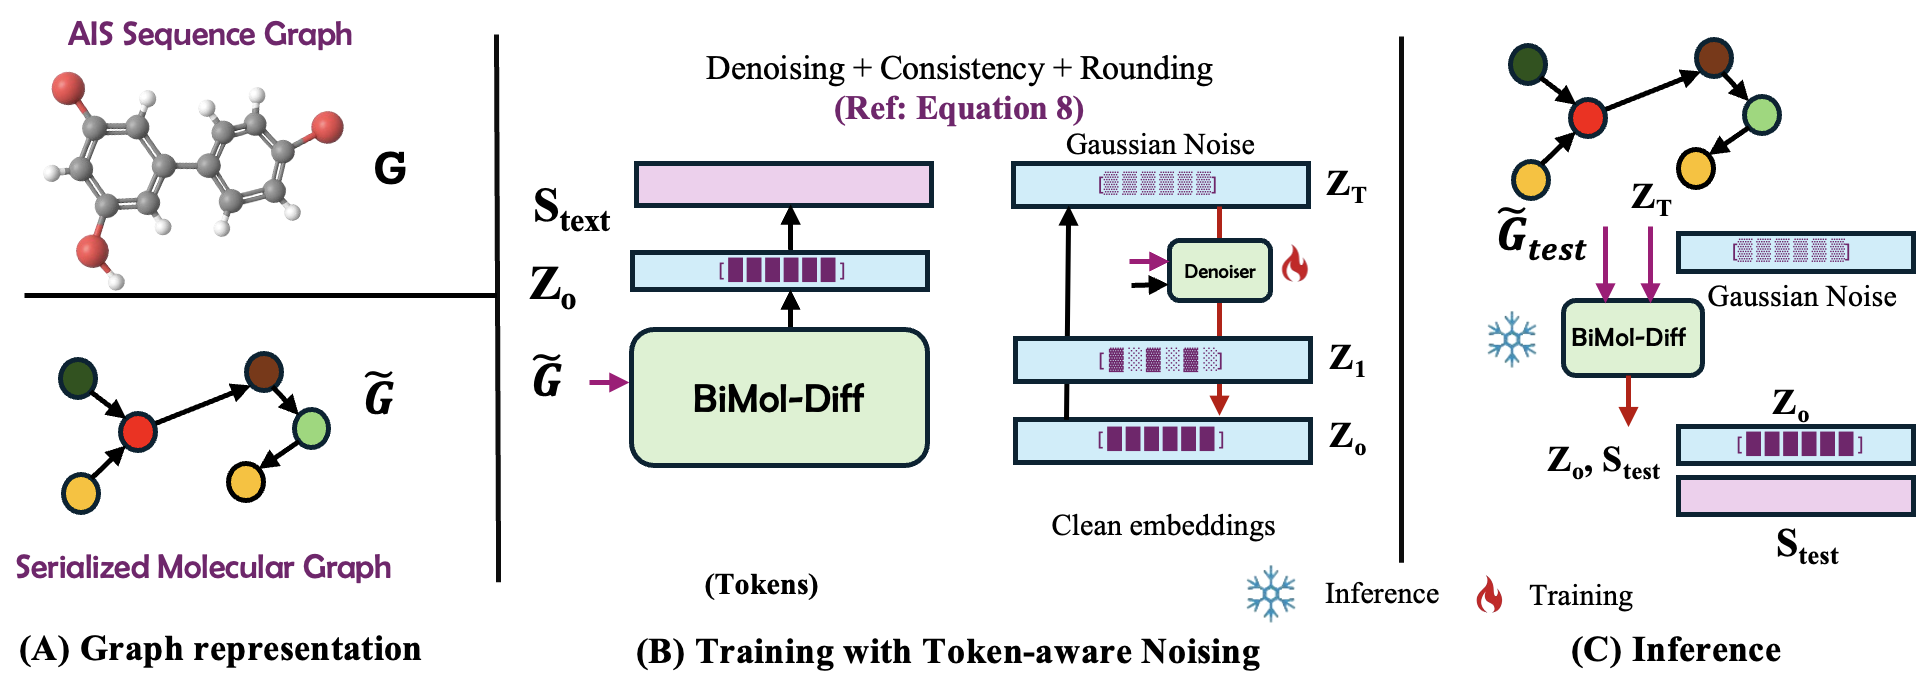
\includegraphics[width=0.8\linewidth]{latex/Images/framework.png}
    \caption{\textbf{The \texttt{BiMol-Diff} Framework.} (A) Molecules are represented through canonical SMILES, AIS-aware tokens, and serialized graph-triplet sequences. (B) \textbf{Training:} the model is trained with token-aware noising that preserves chemically salient tokens, optimizing denoising, consistency, and rounding objectives. (C) \textbf{Inference:} starting from Gaussian noise, iterative denoising and rounding generate either a caption (G2S) or a serialized molecular graph sequence (S2G), which is then deterministically decoded into canonical SMILES.}
    \label{framework}
    \vspace{-4mm}
\end{figure*}

\subsubsection{Diffusion Models: Forward and Reverse Process}

\noindent Denoising diffusion probabilistic models (DDPMs) are generative models that learn a data distribution, often conditioned on some context $\mathbf{c}$, $p(\mathbf{z}_0 \mid \mathbf{c})$. They consist of a fixed forward process and a learned reverse process.

\noindent \textbf{Forward process}: A standard DDPM forward process corrupts clean data $\mathbf{z}_0$ through a Markov chain with noise-schedule coefficients $\{\alpha_t\}_{t=1}^T$ controlling signal decay. This yields the standard closed-form for sampling a noised state $\mathbf{z}_t$ at timestep $t$:
\begin{equation}
    \mathbf{z}_t = \sqrt{\bar{\alpha}_t}\,\mathbf{z}_0 + \sqrt{1 - \bar{\alpha}_t}\,\boldsymbol{\epsilon},
\end{equation}
with $\quad \bar{\alpha}_t = \prod_{s=1}^t \alpha_s \text{ and } \boldsymbol{\epsilon}\sim\mathcal{N}(\mathbf 0,\mathbf I)$. Standard diffusion models typically use a fixed, data-agnostic (isotropic) noise schedule.

\noindent \textbf{Reverse process with Conditional Denoising}: The reverse process learns to recover the clean data $\mathbf{z}_0$ from pure noise $\mathbf{z}_T \sim \mathcal{N}(\mathbf 0,\mathbf I)$. It is defined as a Markov chain $p_\theta(\mathbf{z}_{0:T})$ where each reverse transition $p_\theta(\mathbf{z}_{t-1} \mid \mathbf{z}_t, \mathbf{c})$ is a Gaussian whose mean $\boldsymbol{\mu}_\theta$ and variance $\boldsymbol{\Sigma}_\theta$ are parameterized by a model $\mathcal{M}_\theta(\mathbf{z}_t, t, \mathbf{c})$. The model is trained to predict the mean of the true posterior $q(\mathbf{z}_{t-1} \mid \mathbf{z}_t, \mathbf{z}_0)$. The model parameters $\theta$ are optimized by maximizing the variational lower bound (VLB) on the conditional log-likelihood:
\begin{equation}
\resizebox{\columnwidth}{!}{
$
\begin{aligned}
\mathcal{L}_{\text{vlb}} 
= \mathbb{E}_{q} \Big[
    &\underbrace{-\log p_\theta(\mathbf{z}_0 \mid \mathbf{z}_1, \mathbf{c})}_{\text{Reconstruction } (L_0)} \\
    & + \sum_{t=2}^{T} 
        \underbrace{D_{\mathrm{KL}}\!\left(
            q(\mathbf{z}_{t-1} \mid \mathbf{z}_t, \mathbf{z}_0)
            \,\big\|\,
            p_\theta(\mathbf{z}_{t-1} \mid \mathbf{z}_t, \mathbf{c})
        \right)}_{\text{Denoising Matching } (L_{t-1})} \\
    &+
        \underbrace{D_{\mathrm{KL}}\!\left(
            q(\mathbf{z}_T \mid \mathbf{z}_0)
            \,\big\|\,
            p(\mathbf{z}_T)
        \right)}_{\text{Prior Matching } (L_T)}
\Big].
\end{aligned}
$
}
\end{equation}

\noindent While this formulation is tractable, direct optimization of the full VLB is often unstable.

\subsubsection{Molecules as Graphs:} \label{MAG}A molecule is represented as a graph
$\mathcal{G} = (\mathbf{V}, \mathbf{X}, \mathbf{A}, \mathbf{P})$, 
where $\mathbf{V} = \{1, \dots, n\}$ is the set of atoms (nodes) and $|\mathbf{V}| = n$.
The atom feature matrix $\mathbf{X} \in \mathbb{R}^{n \times a}$ contains
an $a$-dimensional feature vector for each atom.
The adjacency tensor $\mathbf{A} \in \mathbb{R}^{n \times n \times b}$
encodes bond existence and bond types, where
$\mathbf{A}_{ij:} \in \{0,1\}^b$ indicates the type of the bond between atoms $i$ and $j$.
The coordinate matrix $\mathbf{P} \in \mathbb{R}^{n \times 3}$ stores the 3D
positions of atoms.
Here, $a$ is the atom feature dimension and $b$ is the bond type.
Depending on the task, subsets of these components may be used, e.g.,
$(\mathbf{V}, \mathbf{X}, \mathbf{A})$ for 2D graphs or $(\mathbf{V}, \mathbf{X}, \mathbf{P})$
for 3D conformations.